\subsubsection*{Problem definition}

The aim of this example is to simulate the mass transport with the influence of decay, but without any sorption. At the left side of the considered aquifer there is a volume source of 0.1~m$^3$/d, at the right side there is a constant water pressure of 20 kPa. The tracer substance in the source volume is distributed by a stationary flow in the homogeneous aquifer. The mass distribution after 100 days has to be calculated. Figure \ref{fig51} shows a sketch of the calculation area.

\begin{figure}[htbp]
\centering
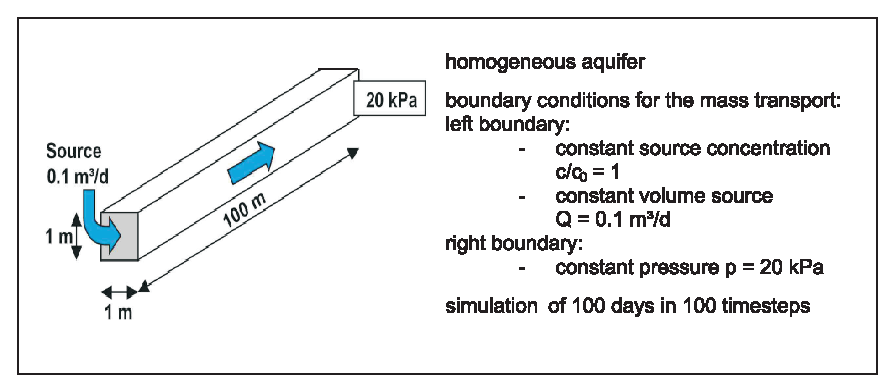
\includegraphics[width=1.0\textwidth]{C/figures/fig51.eps}
\caption{Calculation area: homogeneous aquifer}
\label{fig51}
\end{figure}

\textsl{Assumptions}

\begin{tabbing}
Component: \= no sorption, exclusively decay \\
Aquifer: \> homogeneous, saturated, stationary flow \\
\end{tabbing}

\subsubsection*{Model set-up of the 1~D numerical model}

For the 1-dimensional calculation the calculation area is simplified as a line of a length of 100~m with 100 elements and 101 nodes. As boundary conditions the relative concentration amounts 1 and the source volume of the fluid phase with 0.1~m$^3$/d is given at the left border of the calculation area and a constant pressure of 20 kPa at the right boundary. The used parameters of the soil are listed in table \ref{tab51}. The calculation is divided into 100 time steps with a constant time step length of 1 day. That means, the flow and transport processes in the aquifer within 100 days are simulated.

\begin{table}[htbp]
\centering
\begin{tabular}{|l|l|l|}
\hline
parameter & value & unit \\
\hline
porosity $\Phi$  & 0.2 &  --  \\			
\hline
permeability $K$ & 1.0$\cdot 10^{-12}$ & m$^2$ \\
\hline
density water $\rho$ & 1000 & kg$\cdot m^3$ \\
\hline
viscosity water $\eta$ & 0.001 & Pa$\cdot s$ \\
\hline
dispersion length $\alpha_l$ & 5.0 & m \\
\hline
decay in solved phase $\lambda$ & 2.0$\cdot 10^{-7}$ & s$^{-2}$ \\
\hline
\end{tabular}
\caption{Used parameters}
\label{tab51}
\end{table}

\subsubsection*{Evaluation method}
The concentration distribution at a special point in time and over a given distance is calculated by equation \ref{eq53}. Hereby the retardation coefficient is set equal to 1. The analytical solutions are depicted in figure \ref{fig52} as single symbols.

\subsubsection*{Results}

In figure \ref{fig52} you can find the concentration distribution over the whole length of the 1~D model at the final simulation time of 100 days. Obviously, the numerical results meet well the analytical solutions.

\begin{figure}[htbp]
\centering
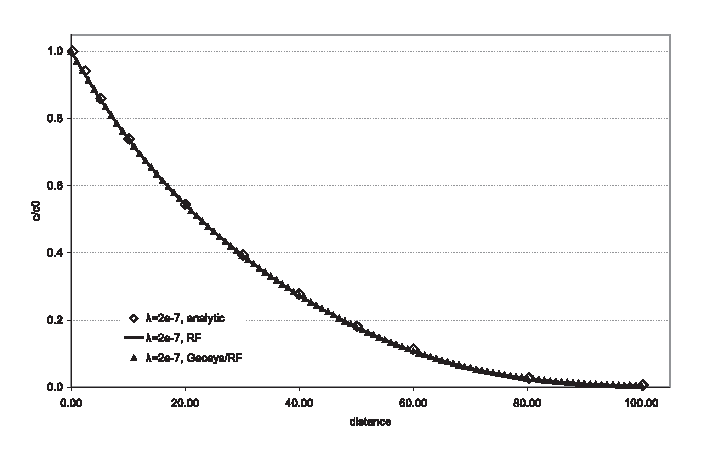
\includegraphics[width=0.8\textwidth]{C/figures/fig52.eps}
\caption{Concentration distribution after 100~d (decay)}
\label{fig52}
\end{figure}

\begin{tabular}{|l|l|l|}
\hline
Benchmark & Problem type	& Path in benchmark deposit \\
\hline	
hc\_decay\_1Du	& HC	& benchmarks $\backslash$HC$\backslash$decay \\
\hline	
\end{tabular}

